\documentclass[11pt]{article}

% Font / typography
\usepackage[T1]{fontenc}
\usepackage{mathpazo}       % Palatino text + math (no external deps)
\usepackage[margin=1in]{geometry}

% Math
\usepackage{amsmath,amssymb,amsthm,mathtools}
\usepackage{enumitem}

% Figures / tables
\usepackage{graphicx}
\usepackage{booktabs}
\usepackage[section]{placeins}   % For \FloatBarrier
\usepackage{eso-pic}

% Preprint-style side identifier on the first page
\newcommand{\preprintnotice}{%
  \AddToShipoutPictureFG*{%
    \AtPageLowerLeft{%
      \put(\LenToUnit{0.30in},\LenToUnit{0.70in}){%
        \rotatebox{90}{\large\color{gray!72}\sffamily
          DOI: 10.5281/zenodo.21325880\hspace{1.2em}[Preprint]\hspace{1.2em}12 Jul 2026}%
      }%
    }%
  }%
}

% Refs
\usepackage{xcolor}
\usepackage{tikz}
\usepackage[colorlinks=true, linkcolor=blue!50!black, citecolor=blue!50!black,
            urlcolor=blue!50!black]{hyperref}
\hypersetup{
  pdftitle={On the Expected Coprime Density of the Least Common Multiple of Random Integers},
  pdfauthor={Muhamad Wakid},
  pdfsubject={Preprint, 12 July 2026. DOI: 10.5281/zenodo.21325880},
  pdfkeywords={random LCM, Euler totient, Mertens product, probabilistic number theory, coprime density, Mobius inversion}
}

% Clickable ORCID mark shown as a superscript beside the author name
\definecolor{orcidgreen}{HTML}{A6CE39}
\newcommand{\orcidmark}{%
  \href{https://orcid.org/0009-0008-6274-778X}{%
    \raisebox{0.55ex}{%
      \tikz[baseline=-0.5ex]{%
        \fill[orcidgreen] (0,0) circle (0.92ex);%
        \node[font=\sffamily\bfseries\fontsize{5}{5}\selectfont,text=white]
          at (0,0) {iD};%
      }%
    }%
  }%
}

% Theorem environments
\newtheorem{theorem}{Theorem}
\newtheorem{proposition}[theorem]{Proposition}
\newtheorem{lemma}[theorem]{Lemma}
\newtheorem{corollary}[theorem]{Corollary}
\theoremstyle{remark}
\newtheorem{remark}[theorem]{Remark}

% Macros
\newcommand{\lcm}{\operatorname{lcm}}
\newcommand{\gcdop}{\operatorname{gcd}}
\newcommand{\PP}{\mathbb{P}}
\newcommand{\EE}{\mathbb{E}}
\newcommand{\one}{\mathbf{1}}
\newcommand{\PM}{\mathcal{P}_M}
\DeclareMathOperator{\Var}{Var}
\DeclareMathOperator{\Cov}{Cov}
\DeclareMathOperator{\Li}{Li}

\title{On the Expected Coprime Density of the\\[2pt]
Least Common Multiple of Random Integers}
\author{Muhamad Wakid\,\orcidmark}
\date{}

\begin{document}

\preprintnotice
\maketitle
\thispagestyle{plain}

\begin{abstract}
Let $X_1, X_2, \ldots$ be independent and identically distributed random variables uniform on $\{2, 3, \ldots, M\}$, and let $L_k = \lcm(X_1, \ldots, X_k)$. We study the expected coprime density
\[
\rho_k(M) = \EE\!\left[\frac{\varphi(L_k)}{L_k}\right],
\]
where $\varphi$ is the Euler totient function. We establish an exact finite-sum identity for $\rho_k(M)$, written as a sum over subsets of primes $p \leq M$ and obtained by M\"obius inversion on the subset lattice. The identity implies $\rho_k(M) \to P_M := \prod_{p \leq M}(1 - 1/p)$ as $k \to \infty$ with $M$ fixed, with a sharp asymptotic equivalence $\rho_k(M) - P_M = P_M \Sigma_k(M)(1 + o(1))$ at geometric rate, where $\Sigma_k(M) = \sum_{p \leq M} q_p(M)^k/(p-1)$ and $q_p(M) = 1 - \lfloor M/p\rfloor/(M-1)$. In the joint regime $k = \lfloor cM \rfloor$, $M \to \infty$ (fixed $c > 0$), we prove the full asymptotic equivalence
\[
\ln M \cdot \frac{\rho_{\lfloor cM \rfloor}(M) - P_M}{P_M} \;\longrightarrow\; A(c) := \sum_{j \geq 1} e^{-cj} \ln\!\left(1 + \tfrac{1}{j}\right),
\]
strengthening the leading-order statement to an $o(1)$ remainder by decomposing the multi-prime correction according to subset cardinality and applying a geometric-mean inequality for subset densities. Numerical computation to $M = 10^7$ across $15$ values of $c \in [0.05, 15]$ illustrates the finite-$M$ behaviour; linear extrapolation in $1/\ln M$ agrees with $A(c)$ to within approximately $0.5\%$ for $c \in [0.1, 5]$ and $1.5\%$ over the full tested range. The regime studied here complements earlier random-LCM models by combining i.i.d. sampling with replacement, the observable $\varphi(L_k)/L_k$, and the fixed-support and diagonal scalings considered below.
\end{abstract}

\noindent\textbf{Keywords:} Random LCM, Euler totient, Mertens product, Meissel--Mertens constant, probabilistic number theory, coprime density, M\"obius inversion, Rosser--Schoenfeld bounds.

\noindent\textbf{MSC 2020:} 11N37, 11K65, 11A25.

\section{Introduction}

The least common multiple of random integers is a classical object. Ces\`aro~\cite{Cesaro1885} studied $\gcd$-averages for uniform random pairs. For two independent uniform draws from $\{1,\ldots,n\}$, the classical pair formula gives $\EE[\lcm(X_1,X_2)] \sim \zeta(3)n^2/(4\zeta(2))$ as $n \to \infty$~\cite{HilberdinkToth2016}. The subject has seen substantial recent development. Cilleruelo, Ru\'e, \v{S}arka, and Zumalac\'arregui~\cite{CilleruleoRueSarkaZumalacarregui2014} established almost-sure asymptotics for $\log \lcm$ of random subsets of $\{1, \ldots, n\}$; Fern\'andez and Fern\'andez~\cite{FernandezFernandez2013} studied the distributions and moments of the gcd and lcm of random $r$-tuples, and later surveyed divisibility properties of random samples~\cite{FernandezFernandez2021}; Hilberdink and T\'oth~\cite{HilberdinkToth2016} obtained the average value of $\lcm$ of $k$ integers; Alsmeyer, Kabluchko, and Marynych~\cite{AlsmeyerKabluchkoMarynych2019} proved limit theorems for $\log \lcm$ of random sets; Bostan, Marynych, and Raschel~\cite{BostanMarynychRaschel2019} established distributional convergence of $f(L_n(k))/n^{rk}$ for multiplicative functions $f$ of polynomial growth, where $L_n(k) = \lcm(X_1, \ldots, X_k)$ with $X_i$ uniform on $\{1, \ldots, n\}$ and $k$ fixed as $n \to \infty$; Buraczewski, Iksanov, and Marynych~\cite{BuraczewskiIksanovMarynych2022} established a central limit theorem for $\log \lcm$ of a uniformly sampled $m$-tuple; Iksanov, Marynych, and Raschel~\cite{IksanovMarynychRaschel2022} extended to hyperbolic regions; Kabluchko, Marynych, and Raschel~\cite{KabluchkoMarynychRaschel2023} to broader domains; and Sanna~\cite{Sanna2021} to $q$-analogues. A dissection of Mertens' prime product formula along a different axis (number of prime factors of summand integers) was given by Lichtman~\cite{Lichtman2021}.

The literature includes several distinct sampling regimes: fixed-size random tuples as the support grows, Bernoulli random subsets whose cardinality grows with the support, and uniformly sampled tuples in joint limits. The present paper instead focuses on i.i.d. sampling with replacement from $\{2, \ldots, M\}$, first with fixed support and $k \to \infty$, and then in the diagonal regime $k = \lfloor cM \rfloor$ with $M \to \infty$. The natural object of study in these regimes is not the LCM itself --- which almost surely equals $\lcm(1, \ldots, M)$ for large $k$ at fixed $M$ --- but the arithmetic function
\[
\frac{\varphi(L_k)}{L_k} = \prod_{p \mid L_k}\!\left(1 - \frac{1}{p}\right),
\]
which measures the density of integers coprime to $L_k$. This quantity takes values in $(0, 1]$ and its large-$k$ behaviour is governed by exactly which primes $p \leq M$ appear as divisors of $L_k$. One expects the Mertens product as the limit, and this paper makes that expectation precise with explicit convergence rates. Second-order fluctuations --- the variance asymptotic and a central limit theorem for the centred log coprime density --- are developed in separate work in preparation.

\subsection{Main results}
Throughout, fix an integer $M \geq 2$. Let $X_1, X_2, \ldots$ be i.i.d.\ uniform on $\{2, 3, \ldots, M\}$, set $L_k = \lcm(X_1, \ldots, X_k)$, and write $\rho_k(M) = \EE[\varphi(L_k)/L_k]$. We exclude $1$ because it is inert under the least common multiple. Including it would only add null draws. On $\{1,\ldots,M\}$, for example, $q_p(M)$ would become $1-\lfloor M/p\rfloor/M$; the underlying prime-appearance mechanism is unchanged. Also let $\PM = \{p : p \leq M\}$, $m_p = \lfloor M/p \rfloor$, and
\[
q_p(M) = 1 - \frac{m_p}{M-1},
\]
the probability that a single uniform draw from $\{2, \ldots, M\}$ is not a multiple of $p$. For $T \subseteq \PM$, let
\[
\beta_T(M) = \frac{1}{M-1}\,\Bigl|\bigl\{n \in \{2, \ldots, M\} : \gcdop\bigl(n, \textstyle\prod_{p \in T} p\bigr) = 1\bigr\}\Bigr|.
\]
The Mertens product up to $M$ is $P_M := \prod_{p \leq M}(1 - 1/p)$.

\begin{theorem}[Exact identity]\label{thm:identity}
For every $M \geq 2$ and every $k \geq 1$,
\begin{equation}\label{eq:identity}
\rho_k(M) = P_M \sum_{T \subseteq \PM} \beta_T(M)^k \prod_{p \in T} \frac{1}{p-1}.
\end{equation}
\end{theorem}

\begin{theorem}[Limit and rate]\label{thm:limit-rate}
Let $\Sigma_k(M) := \sum_{p \leq M} q_p(M)^k/(p-1)$ and $\Lambda(M) := \sum_{p \leq M} 1/(p-1)$. For every fixed $M \geq 2$, $\lim_{k \to \infty} \rho_k(M) = P_M$, and
\begin{equation}\label{eq:decomp}
\frac{\rho_k(M) - P_M}{P_M} = \Sigma_k(M) + R_k(M),
\end{equation}
where $R_k(M) \geq 0$ satisfies
\begin{equation}\label{eq:Rk-bound}
R_k(M) \leq \frac{1}{2}\,\Sigma_{k/2}(M)^2 \, e^{\Lambda(M)}.
\end{equation}
In particular $R_k(M) \to 0$ and $\Sigma_k(M) \to 0$ as $k \to \infty$, establishing $\rho_k(M) \to P_M$.
\end{theorem}

\begin{remark}\label{rem:sharp-fixed-M}
The bound~\eqref{eq:Rk-bound} establishes $R_k(M) \to 0$ at exponential rate at fixed $M$, but as an asymptotic equivalence it gives only $R_k(M) = O(\Sigma_{k/2}(M)^2)$, which at fixed $M$ is $O(1) \cdot \Sigma_k(M)$ rather than $o(1)\cdot \Sigma_k(M)$. A tempting independence bound, $\beta_T(M) \leq \prod_{p \in T} q_p(M)$, would give the sharper conclusion but fails on the finite sampling space. For example, at $(M,T)=(17,\{3,5\})$, direct enumeration gives $\beta_T=9/16$ while $q_3q_5=(11/16)(13/16)=143/256$; the events $\{p\mid X\}$ are not independent. The worst violation observed over $M\leq 50$ is $1/90$ at $(M,T)=(31,\{2,3,7\})$. The proof below instead combines the elementary geometric-mean estimate of Lemma~\ref{lem:geom-mean} with a decomposition by $|T|$ and a uniform summation argument.
\end{remark}

\begin{theorem}[Sharp form at fixed $M$]\label{thm:sharp-fixed-M}
For fixed $M \geq 3$, define
\[
q^{*}(M) := \max_{p \leq M} q_p(M),
\qquad
q^{**}(M) := \max_{\substack{T \subseteq \PM\\ |T| \geq 2}} \beta_T(M).
\]
Then $q^{**}(M) < q^{*}(M)$ and, as $k \to \infty$,
\begin{equation}\label{eq:sharp-fixed-M}
\frac{R_k(M)}{\Sigma_k(M)} = O_M\!\left(\left(\frac{q^{**}(M)}{q^{*}(M)}\right)^{\!k}\right),
\end{equation}
where the subscript in $O_M$ records that the implicit constant may depend on the fixed value of $M$. In particular $R_k(M) = o(\Sigma_k(M))$ as $k \to \infty$, and
\[
\rho_k(M) - P_M = P_M\, \Sigma_k(M)\,\bigl(1 + o(1)\bigr) \qquad (k \to \infty,\; M \text{ fixed}).
\]
Moreover, for $M \geq 11$, Ramanujan's strengthening of Bertrand's postulate~\cite{Ramanujan1919} guarantees at least two primes in $(M/2, M]$. Consequently, $q^{**}(M) = (M-3)/(M-1)$ and $q^{*}(M) = (M-2)/(M-1)$, so that $q^{**}(M)/q^{*}(M) = (M-3)/(M-2)$ and the rate of convergence is explicit.
\end{theorem}

\begin{theorem}[Joint scaling, sharp form]\label{thm:joint-sharp}
For each fixed $c > 0$,
\begin{equation}\label{eq:sigma-limit}
\lim_{M \to \infty} \ln M \cdot \Sigma_{\lfloor cM \rfloor}(M) = A(c),
\end{equation}
where
\begin{equation}\label{eq:A-def}
A(c) := \sum_{j \geq 1} e^{-cj} \ln\!\left(1 + \frac{1}{j}\right),
\end{equation}
and moreover
\begin{equation}\label{eq:sharp}
\lim_{M \to \infty} \ln M \cdot \frac{\rho_{\lfloor cM \rfloor}(M) - P_M}{P_M} = A(c).
\end{equation}
\end{theorem}

The leading-order assertion~\eqref{eq:sigma-limit} is established via Mertens' second theorem, Rosser--Schoenfeld bounds, and dominated convergence. The sharp form~\eqref{eq:sharp} is obtained by combining the elementary geometric-mean bound of Lemma~\ref{lem:geom-mean} with a decomposition of the multi-prime correction by subset cardinality and a uniform summation argument.

\begin{proposition}[Asymptotic behaviour of $A$]\label{prop:A-asymptotics}
The function $A \colon (0, \infty) \to (0, \infty)$ is smooth, strictly decreasing, and strictly convex. Moreover:
\begin{enumerate}[label=(\roman*), leftmargin=2em]
\item As $c \to 0^+$,
\[
A(c) = -\ln c - \gamma - \frac{c \ln c}{2} + O(c),
\]
where $\gamma$ is the Euler--Mascheroni constant.
\item As $c \to \infty$,
\[
A(c) = e^{-c} \ln 2 + e^{-2c} \ln \tfrac{3}{2} + e^{-3c}\ln\tfrac{4}{3} + O(e^{-4c}).
\]
\end{enumerate}
\end{proposition}

\subsection{Organisation}
Section~\ref{sec:prelim} fixes notation and records elementary lemmas, including the geometric-mean bound Lemma~\ref{lem:geom-mean}. Sections~\ref{sec:thm1},~\ref{sec:thm2},~\ref{sec:thm-sharp-fixed-M}, and~\ref{sec:thm4} prove Theorems~\ref{thm:identity},~\ref{thm:limit-rate},~\ref{thm:sharp-fixed-M}, and~\ref{thm:joint-sharp} respectively. Section~\ref{sec:numerics} presents numerical evidence. Section~\ref{sec:discussion} discusses the fluctuations problem and other extensions. Section~\ref{sec:conclusion} concludes.

\section{Preliminaries}\label{sec:prelim}

Notation is standard: $\varphi$ is Euler's totient, $p$ ranges over primes, $\mathcal{P}(n) = \{p : p \mid n\}$, and $\PM = \{p : p \leq M\}$. We use $\ln$ (natural logarithm) throughout; the Mertens product is $P_M = \prod_{p \leq M}(1 - 1/p)$.

For $p \in \PM$, every multiple of $p$ in $\{1, \ldots, M\}$ also lies in $\{2, \ldots, M\}$ since $p \geq 2$, so $m_p = \lfloor M/p \rfloor$ equals the number of multiples of $p$ in the sampling space. For $T \subseteq \PM$, let $A_T(M) = \{n \in \{2, \ldots, M\} : \gcdop(n, \prod_{p \in T} p) = 1\}$, so $\beta_T(M) = |A_T(M)|/(M-1)$, $\beta_\emptyset(M) = 1$, and $\beta_{\{p\}}(M) = q_p(M)$.

\begin{lemma}\label{lem:betaT-power}
For any $T \subseteq \PM$,
\[
\PP\bigl(\forall i \leq k,\; X_i \in A_T(M)\bigr) = \beta_T(M)^k,
\]
equivalently, $\PP(\text{no prime in $T$ divides $L_k$}) = \beta_T(M)^k$.
\end{lemma}
\begin{proof}
Immediate from independence of $X_1, \ldots, X_k$ and the fact that $p \mid L_k$ iff $p \mid X_i$ for some $i$.
\end{proof}

\begin{lemma}\label{lem:single-prime}
For any $\emptyset \neq T \subseteq \PM$ and any $p_0 \in T$, $\beta_T(M) \leq q_{p_0}(M)$.
\end{lemma}
\begin{proof}
$A_T(M) \subseteq \{n \in \{2, \ldots, M\} : p_0 \nmid n\}$.
\end{proof}

\begin{lemma}[Two-prime bound for $|T| \geq 2$]\label{lem:two-prime}
Let $T \subseteq \PM$ with $|T| \geq 2$, and let $p_0, p_1$ be any two distinct elements of $T$. Then for every $k \geq 1$,
\[
\beta_T(M)^k \leq q_{p_0}(M)^{k/2}\, q_{p_1}(M)^{k/2}.
\]
\end{lemma}
\begin{proof}
By Lemma~\ref{lem:single-prime} applied to each of $p_0, p_1$, $\beta_T(M)^{k/2} \leq q_{p_0}(M)^{k/2}$ and $\beta_T(M)^{k/2} \leq q_{p_1}(M)^{k/2}$. Multiply.
\end{proof}

\begin{lemma}[Geometric-mean bound for $|T| \geq 1$]\label{lem:geom-mean}
Let $T \subseteq \PM$ with $|T| = r \geq 1$. For every real $k > 0$,
\begin{equation}\label{eq:geom-mean}
\beta_T(M)^k \leq \prod_{p \in T} q_p(M)^{k/r}.
\end{equation}
\end{lemma}
\begin{proof}
By Lemma~\ref{lem:single-prime}, $\beta_T(M) \leq q_p(M)$ for every $p \in T$. Multiplying these $r$ inequalities gives $\beta_T(M)^r \leq \prod_{p \in T} q_p(M)$, and taking both sides to the positive real power $k/r$ preserves the inequality since both sides lie in $[0, 1]$. Rewriting the right-hand side as $\prod_{p \in T} q_p(M)^{k/r}$ gives~\eqref{eq:geom-mean}.
\end{proof}

\begin{remark}[Real-exponent extension of $\Sigma_k$]\label{rem:sigma-real}
Although $\Sigma_k(M) = \sum_{p \leq M} q_p(M)^k/(p-1)$ was introduced at integer $k$ in Theorem~\ref{thm:limit-rate}, the same formula with $k$ replaced by a real exponent $s>0$ defines $\Sigma_s(M)$. Set $\Sigma_0(M):=\Lambda(M)$ by convention. Since $q_p(M)\in[0,1]$, the function $s\mapsto\Sigma_s(M)$ is nonincreasing on $[0,\infty)$ and $\Sigma_s(M)\leq\Lambda(M)$ uniformly for $s\geq0$. The sharp-form proof of Theorem~\ref{thm:joint-sharp} applies $\Sigma_s$ at $s=k/r$ with $r\geq2$; for integer $k$ this exponent is generally non-integer.
\end{remark}

\begin{remark}\label{rem:why-geom-mean}
The estimate in Lemma~\ref{lem:geom-mean} is elementary; its importance here is structural. It permits the multi-prime correction to be stratified by $|T|=r$, replacing the wasteful factor $e^{\Lambda(M)}$ in~\eqref{eq:Rk-bound} by bounds involving $\Sigma_{k/r}(M)^r/r!$. The resulting cardinality decomposition, together with uniform control as $r$ grows, is the main step in proving the sharp joint-scaling form~\eqref{eq:sharp}.
\end{remark}

\section{Proof of Theorem~\ref{thm:identity}}\label{sec:thm1}

For each $S \subseteq \PM$, let $E_S = \{\mathcal{P}(L_k) = \PM \setminus S\}$ be the event that the set of primes dividing $L_k$ is exactly $\PM \setminus S$. On $E_S$,
\begin{equation}\label{eq:phi-over-L-on-ES}
\frac{\varphi(L_k)}{L_k} = \prod_{p \in \PM \setminus S}\!\left(1 - \frac{1}{p}\right) = \frac{P_M}{\prod_{p \in S}(1 - 1/p)} = P_M \prod_{p \in S} \frac{p}{p-1}.
\end{equation}
The events $\{E_S\}_{S \subseteq \PM}$ partition the sample space (primes $> M$ never divide any $X_i$), so
\begin{equation}\label{eq:rho-by-ES}
\rho_k(M) = P_M \sum_{S \subseteq \PM} \PP(E_S) \prod_{p \in S} \frac{p}{p-1}.
\end{equation}
Now $E_S = \{\text{no prime in $S$ divides $L_k$}\} \cap \{\text{every prime in $\PM \setminus S$ divides $L_k$}\}$, so by M\"obius inversion on the subset lattice,
\begin{equation}\label{eq:ES-by-mobius}
\PP(E_S) = \sum_{T \colon S \subseteq T \subseteq \PM} (-1)^{|T|-|S|}\, \PP(\text{no prime in $T$ divides $L_k$}) = \sum_{T \supseteq S} (-1)^{|T|-|S|}\, \beta_T(M)^k,
\end{equation}
by Lemma~\ref{lem:betaT-power}. Substituting~\eqref{eq:ES-by-mobius} into~\eqref{eq:rho-by-ES} and swapping the order of summation,
\[
\rho_k(M) = P_M \sum_{T \subseteq \PM} \beta_T(M)^k \sum_{S \subseteq T} (-1)^{|T|-|S|} \prod_{p \in S} \frac{p}{p-1}.
\]
The inner sum factors over primes in $T$:
\[
\sum_{S \subseteq T} (-1)^{|T|-|S|} \prod_{p \in S} \frac{p}{p-1} = \prod_{p \in T}\!\left(\frac{p}{p-1} - 1\right) = \prod_{p \in T} \frac{1}{p-1}. \qedhere
\]

\section{Proof of Theorem~\ref{thm:limit-rate}}\label{sec:thm2}

Starting from~\eqref{eq:identity} and isolating $T = \emptyset$ (contribution $P_M$),
\[
\frac{\rho_k(M) - P_M}{P_M} = \sum_{T \subseteq \PM,\; T \neq \emptyset} \beta_T(M)^k \prod_{p \in T} \frac{1}{p-1}.
\]
The $|T| = 1$ contributions sum to $\Sigma_k(M)$. Denote the sum of the $|T| \geq 2$ contributions by $R_k(M)$.

To bound $R_k(M)$, group each $T$ with $|T| \geq 2$ by its two smallest primes. For each pair $\{p_0, p_1\}$ with $p_0 < p_1 \in \PM$, let $\mathcal{T}(p_0, p_1) = \{T \subseteq \PM : \min T = p_0,\; \text{second-min}\, T = p_1\}$. Then every $T$ with $|T| \geq 2$ lies in exactly one such class, and $T \in \mathcal{T}(p_0, p_1)$ iff $T = \{p_0, p_1\} \cup U$ for some $U \subseteq \PM \cap (p_1, \infty)$. By Lemma~\ref{lem:two-prime},
\begin{align*}
R_k(M) &= \sum_{p_0 < p_1 \in \PM} \sum_{T \in \mathcal{T}(p_0, p_1)} \beta_T(M)^k \prod_{p \in T} \frac{1}{p-1} \\
&\leq \sum_{p_0 < p_1} \frac{q_{p_0}(M)^{k/2}}{p_0 - 1}\cdot \frac{q_{p_1}(M)^{k/2}}{p_1 - 1} \sum_{U \subseteq \PM \cap (p_1, \infty)} \prod_{p \in U} \frac{1}{p-1} \\
&\leq \sum_{p_0 < p_1} \frac{q_{p_0}(M)^{k/2}}{p_0 - 1}\cdot \frac{q_{p_1}(M)^{k/2}}{p_1 - 1} \cdot e^{\Lambda(M)},
\end{align*}
using
\[
\sum_{U \subseteq \PM \cap (p_1,\infty)} \prod_{p \in U}\frac{1}{p-1}
= \prod_{p \in \PM \cap (p_1,\infty)}\left(1+\frac{1}{p-1}\right)
\leq \prod_{p \leq M}\left(1+\frac{1}{p-1}\right)
\leq e^{\Lambda(M)}.
\]
The inequality $\sum_{p_0 < p_1} a_{p_0} a_{p_1} \leq \tfrac12(\sum_p a_p)^2$ with $a_p = q_p(M)^{k/2}/(p-1)$ gives~\eqref{eq:Rk-bound}.

For the limit: each $q_p(M) < 1$ and $\PM$ is finite, so $\Sigma_k(M) \to 0$ as $k \to \infty$; and $\Sigma_{k/2}(M) \to 0$ similarly, so $R_k(M) \to 0$ by~\eqref{eq:Rk-bound}. Hence $(\rho_k(M) - P_M)/P_M \to 0$, i.e.\ $\rho_k(M) \to P_M$. \qed

\section{Proof of Theorem~\ref{thm:sharp-fixed-M}}\label{sec:thm-sharp-fixed-M}

Recall $R_k(M) = \sum_{T \subseteq \PM,\, |T| \geq 2}\beta_T(M)^k \prod_{p \in T}\frac{1}{p-1}$.

\emph{Step 1: $q^{**}(M) < q^{*}(M)$ for $M \geq 3$.} Fix any $T \subseteq \PM$ with $|T| \geq 2$ and pick distinct $p_0, p_1 \in T$. By Lemma~\ref{lem:single-prime}, $\beta_T(M) \leq q_{p_0}(M) \leq q^*(M)$. We show the first inequality is strict, which gives $\beta_T < q^*$.

Strict inclusion $A_T(M) \subsetneq A_{\{p_0\}}(M)$ holds because $p_1$ itself, viewed as an integer in $\{2, \ldots, M\}$, belongs to $A_{\{p_0\}}(M) \setminus A_T(M)$: indeed $p_1$ is coprime to $p_0$ (distinct primes) so $p_1 \in A_{\{p_0\}}(M)$, but $p_1$ is divisible by $p_1 \in T$ so $p_1 \notin A_T(M)$. Hence $|A_T| < |A_{\{p_0\}}|$, i.e.\ $\beta_T < q_{p_0}$. Since this holds for every $T$ with $|T| \geq 2$, $q^{**}(M) < q^*(M)$.

\emph{Step 2: bound on $R_k$.} For every $T$ with $|T| \geq 2$, $\beta_T \leq q^{**}$, so
\[
R_k(M) = \sum_{|T| \geq 2}\beta_T^k \prod_{p \in T}\frac{1}{p-1} \leq (q^{**})^k \sum_{|T| \geq 2}\prod_{p \in T}\frac{1}{p-1}.
\]
The last sum is at most $\prod_{p \leq M}(1 + 1/(p-1)) = \prod_{p \leq M}p/(p-1) = 1/P_M \leq e^{\Lambda(M)}$ (Mertens). Hence
\begin{equation}\label{eq:Rk-qstarstar}
R_k(M) \leq (q^{**}(M))^k \cdot e^{\Lambda(M)}.
\end{equation}

\emph{Step 3: lower bound on $\Sigma_k$.} Let $p^*$ be any prime with $q_{p^*}(M) = q^*(M)$. Then
\begin{equation}\label{eq:Sigma-qstar}
\Sigma_k(M) \geq \frac{(q^*(M))^k}{p^* - 1} \geq \frac{(q^*(M))^k}{M-1}.
\end{equation}

\emph{Step 4: combining.} Dividing~\eqref{eq:Rk-qstarstar} by~\eqref{eq:Sigma-qstar},
\[
\frac{R_k(M)}{\Sigma_k(M)} \leq (M-1)\, e^{\Lambda(M)}\left(\frac{q^{**}(M)}{q^*(M)}\right)^{\!k}.
\]
Since $q^{**} < q^*$ (Step~1), the right-hand side tends to $0$ geometrically in $k$, establishing~\eqref{eq:sharp-fixed-M}.

\emph{Step 5: explicit rate for $M \geq 11$.} For $M \geq 11$, by Ramanujan's strengthening of Bertrand's postulate~\cite{Ramanujan1919} there are at least two primes in $(M/2, M]$; call them $p_1, p_2$. Both have $m_p = 1$, so $q_{p_i} = (M-2)/(M-1) = q^*$. For $T = \{p_1, p_2\}$, $p_1 p_2 > (M/2)^2 \geq M$ (for $M \geq 4$), so $\lfloor M/(p_1 p_2)\rfloor = 0$ and, by direct inclusion--exclusion, $|A_T(M)| = (M-1)-1-1 = M-3$, so $\beta_T = (M-3)/(M-1)$. To see this is the maximum: any other $T$ with $|T| \geq 2$ satisfies either (i)~$T \subseteq \PM \cap (M/2, M]$, in which case $\beta_T = (M - |T| - 1)/(M-1) \leq (M-3)/(M-1)$ since $|T| \geq 2$; or (ii)~$T$ contains some $p$ with $m_p \geq 2$, in which case $\beta_T \leq q_p \leq (M-3)/(M-1)$ (since $q_p = 1 - m_p/(M-1) \leq (M-3)/(M-1)$). Hence $q^{**}(M) = (M-3)/(M-1)$.
\qed

\section{Proof of Theorem~\ref{thm:joint-sharp}}\label{sec:thm4}

We prove~\eqref{eq:sigma-limit} first and then derive~\eqref{eq:sharp} from Lemma~\ref{lem:geom-mean}.

\subsection[Leading-order convergence of Sigma]{Proof of~\eqref{eq:sigma-limit}: leading-order convergence of $\Sigma$}\label{sec:thm4-leading}

Partition primes by $m_p$-value. A prime $p$ satisfies $m_p = j$ iff $p \in (M/(j+1), M/j]$. For such $p$, $q_p(M) = 1 - j/(M-1)$. Write
\[
S_j(M) := \sum_{p \in \PM \colon m_p = j} \frac{1}{p-1},
\]
so $\Sigma_{\lfloor cM \rfloor}(M) = \sum_{j \geq 1}(1 - j/(M-1))^{\lfloor cM \rfloor}\, S_j(M)$.

\emph{Pointwise limit.} For each fixed $j \geq 1$, using $\ln(1 - x) = -x + O(x^2)$ as $x \to 0$,
\[
\bigl(1 - j/(M-1)\bigr)^{\lfloor cM \rfloor} = \exp\bigl(\lfloor cM \rfloor(-j/(M-1) + O(1/M^2))\bigr) \longrightarrow e^{-cj}.
\]
By the prime number theorem with a classical de la Vall\'ee Poussin error term~\cite[Ch.~I.3]{Tenenbaum2015}, partial summation yields the sharpened form of Mertens' second theorem
\[
\sum_{p \leq x} \frac{1}{p} = \ln \ln x + \beta_1 + E(x), \qquad E(x) = O\bigl(\exp(-\alpha\sqrt{\ln x})\bigr),
\]
uniformly in $x \geq 2$, where $\beta_1 \approx 0.2615$ is the Meissel--Mertens constant and $\alpha > 0$ is an absolute constant (unrelated to the regime parameter $c$); in particular $E(x) = o(1/\ln x)$. Applying this at $x = M/j$ and $x = M/(j+1)$ (which requires $M/(j+1) \geq 2$, i.e.\ $j \leq M/2 - 1$),
\begin{equation}\label{eq:mertens-strip}
\sum_{p \in (M/(j+1),\, M/j]} \frac{1}{p} = \ln\!\frac{\ln(M/j)}{\ln(M/(j+1))} + E(M/j) - E(M/(j+1)).
\end{equation}
For each fixed $j \geq 1$, the error term is $o(1/\ln M)$ as $M \to \infty$. A first-order expansion gives
\[
\ln\!\frac{\ln M - \ln j}{\ln M - \ln(j+1)} = \frac{\ln(1 + 1/j)}{\ln M}\bigl(1 + O_j(1/\ln M)\bigr).
\]
The discrepancy between $\sum 1/(p-1)$ and $\sum 1/p$ over the same interval equals $\sum 1/(p(p-1))$. For each fixed $j \geq 1$ this discrepancy is bounded above by $\sum_{p > M/(j+1)} 1/(p(p-1)) = O\bigl((j+1)/M\bigr)$ (since $\sum_{n > N} 1/(n(n-1)) = 1/N$ over integers), hence of order $O(1/M) = o(1/\ln M)$. Multiplying~\eqref{eq:mertens-strip} by $\ln M$ and taking $M \to \infty$ at fixed $j$,
\begin{equation}\label{eq:Sj-pointwise}
\ln M \cdot S_j(M) \longrightarrow \ln(1 + 1/j) \qquad (M \to \infty)
\end{equation}
for each fixed $j$.

\emph{Uniform tail bound.}

\begin{lemma}[Uniform envelope]\label{lem:envelope}
For all $M \geq 289$ and all $1 \leq j \leq M/17$,
\[
S_j(M) \leq \frac{5.04}{\ln(M/j)}.
\]
In particular, for $1 \leq j \leq M^{1/2}$ and $M \geq 289$, $\ln M \cdot S_j(M) \leq 10.08$ uniformly in $j$.
\end{lemma}
\begin{proof}
By the Rosser--Schoenfeld explicit bounds~\cite{RosserSchoenfeld1962}, for $x \geq 17$, $\pi(x) \leq 1.26\, x/\ln x$; the hypothesis $j \leq M/17$ ensures $M/j \geq 17$. Hence the number of primes in $(M/(j+1), M/j]$ is at most $\pi(M/j) \leq 1.26(M/j)/\ln(M/j)$. Each such prime satisfies $p > M/(j+1) \geq M/(2j)$ (using $j \geq 1$), and for $M \geq 4j$ this gives $p - 1 \geq M/(4j)$, so $1/(p-1) \leq 4j/M$ uniformly over the interval (the hypothesis $j \leq M/17$ implies $M \geq 17j \geq 4j$). Therefore
\[
S_j(M) \leq \pi(M/j) \cdot \frac{4j}{M} \leq 1.26 \cdot \frac{M/j}{\ln(M/j)} \cdot \frac{4j}{M} = \frac{5.04}{\ln(M/j)}.
\]
For $j \leq M^{1/2}$, $\ln(M/j) \geq \tfrac12 \ln M$, giving $\ln M \cdot S_j(M) \leq 10.08$.
\end{proof}

\emph{Dominated convergence.} Combining the pointwise limit~\eqref{eq:Sj-pointwise} with the envelope Lemma~\ref{lem:envelope} and the inequality $(1 - j/(M-1))^{\lfloor cM \rfloor} \leq 2 e^{-cj}$ (valid uniformly for $1 \leq j \leq M^{1/2}$ and $M \geq M_1(c)$), each term in the main range is bounded by $2 \cdot 10.08\, e^{-cj}/\ln M$, and multiplied by $\ln M$ the envelope $20.16\, e^{-cj}$ is summable in $j$. The tail $j > M^{1/2}$ contributes at most
\[
\sum_{j > M^{1/2}}\bigl(1 - j/(M-1)\bigr)^{\lfloor cM \rfloor}\, S_j(M) \leq \Lambda(M)\,\bigl(1 - M^{-1/2}\bigr)^{\lfloor cM \rfloor} = O\bigl(\ln\ln M\cdot e^{-c\sqrt{M}/2}\bigr),
\]
which is super-polynomially small (and $\Lambda(M) = \sum_p 1/(p-1) = O(\ln\ln M)$ by Mertens). By dominated convergence,
\[
\ln M \cdot \Sigma_{\lfloor cM \rfloor}(M) \longrightarrow \sum_{j \geq 1} e^{-cj}\ln(1 + 1/j) = A(c). \qed
\]

\subsection[Sharp joint-scaling form]{Proof of~\eqref{eq:sharp}: the sharp form}\label{sec:thm4-sharp}

Because of~\eqref{eq:sigma-limit}, it suffices to show $\ln M \cdot R_k(M) \to 0$ in the joint regime:
\begin{equation}\label{eq:Rk-sharp}
\lim_{M \to \infty} \ln M \cdot R_k(M) = 0, \qquad k = \lfloor cM \rfloor.
\end{equation}

\emph{Size decomposition.}
Group $R_k(M)$ by $|T|$:
\[
R_k(M) = \sum_{r \geq 2} R_k^{(r)}(M), \qquad R_k^{(r)}(M) := \sum_{T \subseteq \PM,\, |T| = r} \beta_T^k \prod_{p \in T} \frac{1}{p-1}.
\]

\emph{Bound for each fixed $r \geq 2$.}
By Lemma~\ref{lem:geom-mean}, $\beta_T^k \leq \prod_{p \in T} q_p^{k/r}$ for $|T| = r$. Hence
\begin{equation}\label{eq:Rkr-bound}
R_k^{(r)}(M) \leq \sum_{T \colon |T| = r} \prod_{p \in T} \frac{q_p^{k/r}}{p-1} = e_r\!\left(\left\{\tfrac{q_p^{k/r}}{p-1}\right\}_{p \in \PM}\right) \leq \frac{\Sigma_{k/r}(M)^r}{r!},
\end{equation}
where $e_r$ denotes the $r$-th elementary symmetric polynomial and we used the standard inequality $e_r(x_1, \ldots, x_n) \leq (x_1 + \cdots + x_n)^r / r!$ for nonnegative $x_i$.

The strip argument in Section~\ref{sec:thm4-leading} applies, without change, to any real exponent sequence $s_M \geq 0$ satisfying $s_M/M \to d>0$; the pointwise factor then converges to $e^{-dj}$ and the same dominating envelope applies. Taking $s_M=\lfloor cM\rfloor/r$, for which $s_M/M\to c/r$, gives
\begin{equation}\label{eq:sigma-kr}
\ln M \cdot \Sigma_{k/r}(M) \longrightarrow A(c/r) \qquad (M \to \infty),
\end{equation}
for each fixed $r \geq 2$; see also Remark~\ref{rem:sigma-real}.

Combining~\eqref{eq:Rkr-bound} and~\eqref{eq:sigma-kr}, for each fixed $r \geq 2$,
\begin{equation}\label{eq:lnM-Rkr}
\ln M \cdot R_k^{(r)}(M)
\leq \frac{(\ln M \cdot \Sigma_{k/r}(M))^r}{r!\, (\ln M)^{r-1}}
\longrightarrow 0,
\end{equation}
because the numerator converges to $A(c/r)^r$ while $(\ln M)^{r-1} \to \infty$ for every fixed $r \geq 2$.

\emph{Uniform-in-$r$ summability.}
Pointwise vanishing~\eqref{eq:lnM-Rkr} for each fixed $r$ is not sufficient on its own to conclude $\ln M \cdot R_k(M) \to 0$, because $R_k(M) = \sum_{r \geq 2} R_k^{(r)}(M)$ is an infinite sum. We now establish a uniform-in-$r$ estimate sufficient for term-by-term summation.

Set $v := (k/r)/(M-1) = \lfloor cM \rfloor/(r(M-1))$, so for $M$ sufficiently large (depending on $c$) and $r \geq 1$, $v \geq c/(2r)$. Using $q_j^{k/r} = (1 - j/(M-1))^{k/r} \leq e^{-jv}$ and splitting the strip sum at $j = \lfloor M^{1/2} \rfloor$,
\[
\Sigma_{k/r}(M) = \sum_{j \geq 1} S_j(M)\, q_j^{k/r} \leq \sum_{j=1}^{\lfloor M^{1/2}\rfloor} S_j(M)\, e^{-jv} + \Lambda(M)\bigl(1 - M^{-1/2}\bigr)^{k/r}.
\]
For $M \geq 289$ and $1 \leq j \leq M^{1/2}$, Lemma~\ref{lem:envelope} gives $S_j(M) \leq 10.08/\ln M$ uniformly in $j$; hence
\[
\sum_{j=1}^{\lfloor M^{1/2}\rfloor} S_j(M)\, e^{-jv} \leq \frac{10.08}{\ln M} \cdot \frac{e^{-v}}{1 - e^{-v}} \leq \frac{10.08}{\ln M} \cdot \frac{1}{1 - e^{-v}}.
\]
For every $v > 0$, the elementary inequality $1 - e^{-v} \geq v/(1+v)$ gives $1/(1 - e^{-v}) \leq 1 + 1/v \leq 1 + 2r/c$. Meanwhile, for $2 \leq r \leq r_{\max}(M) := M^{1/2}/\ln M$ and $M$ large, $c\sqrt{M}/(2r) \geq (c/2) \ln M$, so $(1 - M^{-1/2})^{k/r} \leq e^{-c\sqrt{M}/(2r)} \leq M^{-c/2}$, and the second sum contributes at most $\Lambda(M)\, M^{-c/2} = o(1/(\ln M)^2)$. Combining, since $1 + 2r/c \leq (2 + 2/c)\, r$ for $r \geq 1$,
\begin{equation}\label{eq:sigma-kr-uniform}
\Sigma_{k/r}(M) \leq \frac{C_u\, r}{\ln M}, \qquad 2 \leq r \leq r_{\max}(M),
\end{equation}
for some constant $C_u = C_u(c)$ (explicitly, $C_u \leq 10.08 (2 + 2/c)$) and $M \geq M_1(c)$.

\emph{Summation over $r$.}
Combining~\eqref{eq:Rkr-bound} and~\eqref{eq:sigma-kr-uniform}, for $2 \leq r \leq r_{\max}(M)$,
\[
R_k^{(r)}(M) \leq \frac{\Sigma_{k/r}(M)^r}{r!} \leq \frac{(C_u r/\ln M)^r}{r!} \leq \left(\frac{C_u e}{\ln M}\right)^{\!r}
\]
where we used Stirling's bound $r! \geq (r/e)^r$. For $r > r_{\max}(M)$, the universal bound $\Sigma_s(M) \leq \Sigma_0(M) = \Lambda(M)$ (valid for any $s \geq 0$ since $q_p \in [0, 1]$) gives
\[
R_k^{(r)}(M) \leq \frac{\Lambda(M)^r}{r!} \leq \left(\frac{e\,\Lambda(M)}{r}\right)^{\!r} \leq \left(\frac{e\,\Lambda(M)\ln M}{M^{1/2}}\right)^{\!r},
\]
which is super-polynomially small in $M$ (since $\Lambda(M)\ln M / M^{1/2} \to 0$) and sums to $o(1/M^{1/3})$ over $r > r_{\max}(M)$. Therefore, for $M$ sufficiently large that $C_u e / \ln M \leq 1/2$,
\begin{equation}\label{eq:Rk-total}
R_k(M) \leq \sum_{r=2}^{\lfloor r_{\max}\rfloor} \left(\frac{C_u e}{\ln M}\right)^{\!r} + o\bigl(1/M^{1/3}\bigr) \leq \frac{2(C_u e)^2}{(\ln M)^2} + o\bigl(1/M^{1/3}\bigr) = O\!\left(\frac{1}{(\ln M)^2}\right).
\end{equation}

\emph{Conclusion.}
From~\eqref{eq:Rk-total}, $\ln M \cdot R_k(M) = O(1/\ln M) \to 0$ as $M \to \infty$, which is~\eqref{eq:Rk-sharp}.

Combining with~\eqref{eq:sigma-limit},
\[
\ln M \cdot \frac{\rho_k - P_M}{P_M} = \ln M \cdot \Sigma_k + \ln M \cdot R_k \longrightarrow A(c) + 0 = A(c),
\]
which is~\eqref{eq:sharp}. \qed

\begin{proof}[Proof of Proposition~\ref{prop:A-asymptotics}]
For every $c_0>0$, the series~\eqref{eq:A-def} and all of its termwise derivatives converge uniformly on $[c_0,\infty)$ by the Weierstrass $M$-test. Thus $A$ is smooth on $(0,\infty)$, and its first two derivatives are
\[
A'(c) = -\sum_{j \geq 1} j\, e^{-cj} \ln(1 + 1/j), \quad A''(c) = \sum_{j \geq 1} j^2\, e^{-cj} \ln(1 + 1/j),
\]
both with every term positive, so $A'(c) < 0$ (strict monotonicity) and $A''(c) > 0$ (strict convexity) for all $c > 0$.

\emph{Proof of (ii).} Isolating the first three terms of~\eqref{eq:A-def} and using $\ln(1 + 1/j)$ is decreasing in $j$,
\[
A(c) - e^{-c} \ln 2 - e^{-2c} \ln \tfrac{3}{2} - e^{-3c}\ln\tfrac{4}{3} = \sum_{j \geq 4} e^{-cj} \ln(1 + 1/j) \leq \ln \tfrac{5}{4} \sum_{j \geq 4} e^{-cj} = \frac{\ln(5/4)}{1 - e^{-c}}\, e^{-4c},
\]
which is $O(e^{-4c})$ as $c \to \infty$ since $1/(1 - e^{-c}) \to 1$.

\emph{Proof of (i).} For every $j \geq 1$, the alternating Taylor series $\ln(1 + x) = \sum_{k \geq 1}(-1)^{k+1} x^k/k$ at $x = 1/j$ gives
\begin{equation}\label{eq:log-Taylor}
\ln(1 + 1/j) = \frac{1}{j} - \frac{1}{2j^2} + R(j), \qquad |R(j)| \leq \frac{1}{3 j^3},
\end{equation}
where the bound on $R(j)$ is the alternating-series remainder. Substituting into~\eqref{eq:A-def} and separating the three resulting convergent series,
\begin{equation}\label{eq:A-decomp}
A(c) = -\ln(1 - e^{-c}) - \tfrac12\, \Li_2(e^{-c}) + \sum_{j \geq 1} e^{-cj} R(j),
\end{equation}
where $\sum_{j \geq 1} e^{-cj}/j = -\ln(1 - e^{-c})$ and $\sum_{j \geq 1} e^{-cj}/j^2 = \Li_2(e^{-c})$.

The sum $\sum_{j \geq 1} R(j)$ converges absolutely by~\eqref{eq:log-Taylor}. Since $\sum_{j=1}^N \ln(1 + 1/j) = \ln(N+1)$ (telescoping), $\sum_{j=1}^N 1/j = H_N = \ln N + \gamma + O(1/N)$, and $\sum_{j=1}^N 1/(2j^2) = \pi^2/12 + O(1/N)$,
\[
\sum_{j=1}^N R(j) = \sum_{j=1}^N \bigl(\ln(1+1/j) - 1/j + 1/(2j^2)\bigr) = \ln(N+1) - H_N + \tfrac12 \sum_{j=1}^N 1/j^2,
\]
which tends to $\pi^2/12 - \gamma$ as $N \to \infty$. Hence
\begin{equation}\label{eq:sum-R}
\sum_{j \geq 1} R(j) = \frac{\pi^2}{12} - \gamma.
\end{equation}
For the $c$-dependence of the third term in~\eqref{eq:A-decomp},
\[
\sum_{j \geq 1} e^{-cj} R(j) - \sum_{j \geq 1} R(j) = -\sum_{j \geq 1}(1 - e^{-cj}) R(j),
\]
whose absolute value is bounded, using $1 - e^{-cj} \leq cj$ and $|R(j)| \leq 1/(3j^3)$, by $(c/3) \sum_{j \geq 1} 1/j^2 = c\pi^2/18$. Hence
\begin{equation}\label{eq:sumR-c}
\sum_{j \geq 1} e^{-cj} R(j) = \frac{\pi^2}{12} - \gamma + O(c).
\end{equation}
Finally, expand the first two terms of~\eqref{eq:A-decomp}. From $1 - e^{-c} = c(1 - c/2 + O(c^2))$,
\begin{equation}\label{eq:log-1-expm}
-\ln(1 - e^{-c}) = -\ln c - \ln(1 - c/2 + O(c^2)) = -\ln c + c/2 + O(c^2).
\end{equation}
For the dilogarithm, the reflection identity $\Li_2(z) + \Li_2(1 - z) = \pi^2/6 - \ln z \ln(1 - z)$ gives, at $z = e^{-c}$,
\[
\Li_2(e^{-c}) = \frac{\pi^2}{6} + c \ln(1 - e^{-c}) - \Li_2(1 - e^{-c}).
\]
Using $\ln(1 - e^{-c}) = \ln c - c/2 + O(c^2)$ (from~\eqref{eq:log-1-expm}) and $\Li_2(u) = u + u^2/4 + O(u^3)$ as $u \to 0$ with $u = 1 - e^{-c} = c - c^2/2 + O(c^3)$,
\begin{equation}\label{eq:Li2-exp}
\Li_2(e^{-c}) = \frac{\pi^2}{6} + c \ln c - c - \frac{c^2}{4} + O(c^3).
\end{equation}
Substituting~\eqref{eq:log-1-expm},~\eqref{eq:Li2-exp}, and~\eqref{eq:sumR-c} into~\eqref{eq:A-decomp},
\[
A(c) = \bigl[-\ln c + c/2\bigr] - \tfrac12\bigl[\tfrac{\pi^2}{6} + c\ln c - c\bigr] + \bigl[\tfrac{\pi^2}{12} - \gamma\bigr] + O(c) = -\ln c - \gamma - \tfrac{c \ln c}{2} + O(c),
\]
where the $c$-linear and $c^2$ remainders are absorbed into $O(c)$.
\end{proof}

\section{Numerical Evidence}\label{sec:numerics}

The theorems in Sections~\ref{sec:thm1}--\ref{sec:thm4} are proved rigorously and require no numerical verification. The numerics below are included to illustrate the finite-$M$ behaviour of the asymptotics in Theorems~\ref{thm:limit-rate}--\ref{thm:joint-sharp}, which may be useful to readers who wish to work with these results computationally. In particular, the $O(1/\ln M)$ convergence in Theorem~\ref{thm:joint-sharp} is slow, and the tables below make the rate of convergence concrete. Computations and code supporting all figures and tables are openly available at the repository cited in Section~\ref{sec:conclusion}.

\emph{Computational protocol.} Exact finite-$M$ identity checks use integer or rational arithmetic. Deterministic prime sums and the series $A(c)$ are evaluated directly in IEEE 754 double precision; no stochastic approximation is used for those quantities. The positive series defining $A(c)$ is truncated adaptively when the next term is below $10^{-17}$. Monte Carlo estimates use NumPy's default random-number generator with $N=2000$ independent replicates per displayed cell and deterministic cell seed $2026+1000M+k$. The statistic $\varphi(L_k)/L_k$ is evaluated from the union of the prime divisors of the sampled integers. Values obtained from Theorem~\ref{thm:identity} in the finite exact checks are computed by direct enumeration over subsets $T \subseteq \PM$. The source bundle contains the scripts, cell-level standard errors, seeds, and raw CSV output.

\emph{Theorem~\ref{thm:identity}.} For $M \in \{5, 6, 7, 8, 9, 10\}$ and $k \in \{2, 3, 4, 5\}$, $\rho_k(M)$ computed via direct enumeration of all $(M-1)^k$ tuples was compared with the right-hand side of~\eqref{eq:identity}, using exact rational arithmetic throughout. All $24$ test cases matched \emph{exactly} as rationals.

\emph{Theorem~\ref{thm:limit-rate}.} Figure~\ref{fig:convergence} shows $\rho_k(M)$ versus $k$ for $M \in \{100,300,1000\}$. Table~\ref{tab:thm2} compares the Monte Carlo gap $\rho_k(M)-P_M$ ($N=2000$) with the deterministic first-order term $P_M\Sigma_k(M)$ obtained by direct prime summation, and lists the cell-specific standard errors.

\begin{figure}[!htbp]
\centering
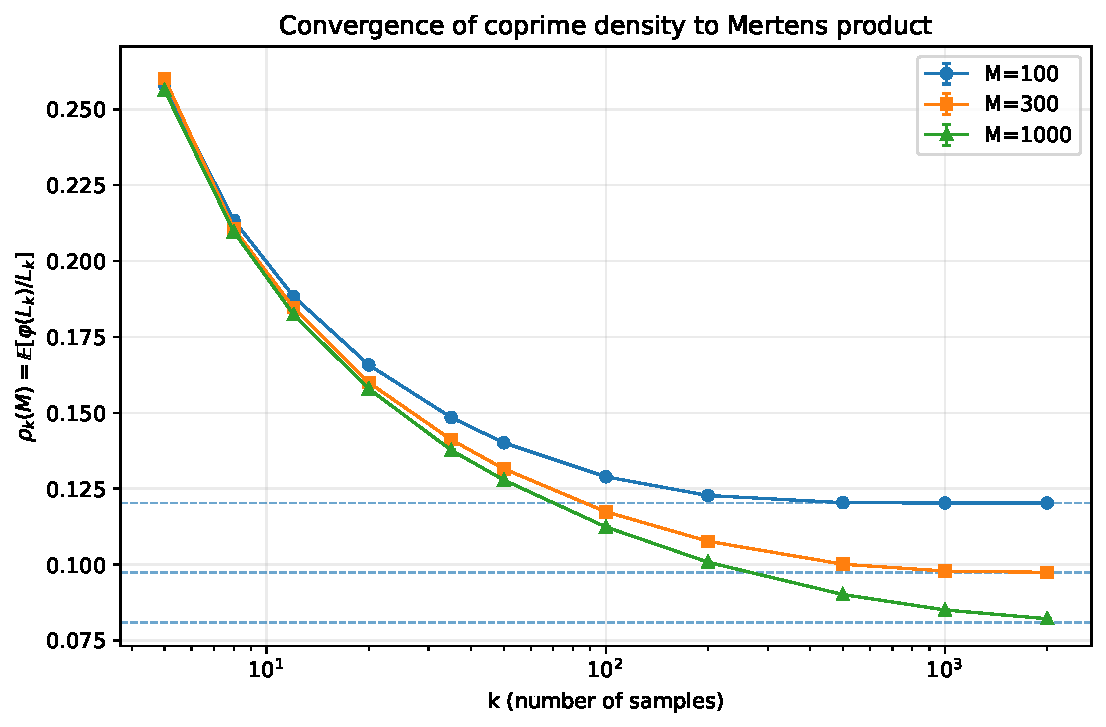
\includegraphics[width=0.85\linewidth]{fig1_convergence.pdf}
\caption{Monte Carlo estimates of $\rho_k(M)$ for $M \in \{100, 300, 1000\}$, based on $N = 2000$ independent replicates per point. Error bars show $\pm 1$ standard error of the sample mean. Dashed lines indicate the exact Mertens product $P_M$.}
\label{fig:convergence}
\end{figure}

\begin{table}[!htbp]
\centering
\caption{Seeded Monte Carlo estimates of $\rho_k(M)-P_M$ ($N=2000$ per cell) compared with the deterministic first-order term $P_M\Sigma_k(M)$. The reported standard errors are cell-specific. The ratio column illustrates the approach to unity predicted by Theorem~\ref{thm:limit-rate}.}
\label{tab:thm2}
\small
\resizebox{\linewidth}{!}{%
\begin{tabular}{rrrrrrrr}
\toprule
$M$ & $k$ & $\rho_k(M)$ (MC) & s.e. & $P_M$ & gap obs. & gap pred. & ratio \\
\midrule
100  & 50   & 0.140151 & $1.41\times10^{-4}$ & 0.120317 & 0.019834 & 0.018552 & 1.069 \\
100  & 200  & 0.122783 & $4.75\times10^{-5}$ & 0.120317 & 0.002465 & 0.002482 & 0.993 \\
300  & 100  & 0.117427 & $7.59\times10^{-5}$ & 0.097459 & 0.019969 & 0.018264 & 1.093 \\
300  & 500  & 0.100147 & $2.43\times10^{-5}$ & 0.097459 & 0.002688 & 0.002642 & 1.018 \\
1000 & 500  & 0.090173 & $2.32\times10^{-5}$ & 0.080965 & 0.009208 & 0.008758 & 1.051 \\
1000 & 2000 & 0.082197 & $8.33\times10^{-6}$ & 0.080965 & 0.001232 & 0.001220 & 1.010 \\
1000 & 5000 & 0.081022 & $1.82\times10^{-6}$ & 0.080965 & 0.000057 & 0.000055 & 1.032 \\
3000 & 5000 & 0.071308 & $4.63\times10^{-6}$ & 0.069966 & 0.001342 & 0.001335 & 1.006 \\
\bottomrule
\end{tabular}%
}
\end{table}

\emph{Theorem~\ref{thm:sharp-fixed-M} (sharp form at fixed $M$).} Table~\ref{tab:sharp-fixed} exhibits $R_k(M)/\Sigma_k(M)$ for $M \in \{20, 30\}$ and $k \in \{20, 40, 80, 160\}$ alongside the geometric rate factor $(q^{**}/q^{*})^k$ from Theorem~\ref{thm:sharp-fixed-M}; the theorem's actual upper bound also contains the fixed prefactor $(M-1)e^{\Lambda(M)}$. The observed ratio decays exponentially, in fact substantially faster than the rate factor alone: at $M=20$, the ratio falls from $4.5 \times 10^{-2}$ at $k=20$ to $1.2 \times 10^{-5}$ at $k=160$, while $(17/18)^{140} \approx 3 \times 10^{-4}$.

\begin{table}[!htbp]
\centering
\caption{Observed ratio $R_k(M)/\Sigma_k(M)$ versus the geometric rate factor $(q^{**}(M)/q^{*}(M))^k$ from Theorem~\ref{thm:sharp-fixed-M}. The full upper bound also contains an $M$-dependent prefactor. For $M \geq 11$, $q^{**}/q^{*} = (M-3)/(M-2)$.}
\label{tab:sharp-fixed}
\small
\begin{tabular}{rrrr}
\toprule
$M$ & $k$ & $R_k/\Sigma_k$ (obs.) & $(q^{**}/q^*)^k$ (rate) \\
\midrule
20 & 20 & $4.52 \times 10^{-2}$ & $3.19 \times 10^{-1}$ \\
20 & 40 & $1.22 \times 10^{-2}$ & $1.02 \times 10^{-1}$ \\
20 & 80 & $1.15 \times 10^{-3}$ & $1.03 \times 10^{-2}$ \\
20 & 160 & $1.18 \times 10^{-5}$ & $1.07 \times 10^{-4}$ \\
\midrule
30 & 20 & $6.30 \times 10^{-2}$ & $4.83 \times 10^{-1}$ \\
30 & 40 & $2.27 \times 10^{-2}$ & $2.34 \times 10^{-1}$ \\
30 & 80 & $4.30 \times 10^{-3}$ & $5.45 \times 10^{-2}$ \\
30 & 160 & $2.20 \times 10^{-4}$ & $2.97 \times 10^{-3}$ \\
\bottomrule
\end{tabular}
\end{table}

\emph{Theorem~\ref{thm:joint-sharp}.} Figure~\ref{fig:joint} plots $\ln M \cdot \Sigma_{\lfloor cM \rfloor}(M)$, evaluated deterministically by direct prime summation in double precision, at $M \in \{10^3, 10^4, 10^5, 10^6\}$ against $A(c)$; Table~\ref{tab:joint} extends to $M = 10^7$ across 15 values of $c \in [0.05, 15]$. The relative error $(\ln M \cdot \Sigma_{\lfloor cM \rfloor}(M) - A(c))/A(c)$ at $M = 10^7$ ranges from approximately $10.7\%$ at $c = 0.05$ down to $2.1\%$ at $c = 15$, decreasing monotonically in $c$; these residuals are consistent with an $O(1/\ln M)$ correction arising from the next-order expansion of the prime-strip difference in~\eqref{eq:mertens-strip}. Linear extrapolation of the sequence $\{\ln M \cdot \Sigma_{\lfloor cM \rfloor}(M)\}_M$ in the variable $1/\ln M$ (fitted over $M \in \{10^4, 10^5, 10^6, 10^7\}$) agrees with $A(c)$ to within approximately $0.5\%$ for $c \in [0.1, 5]$ and to within $1.5\%$ across the full tested range $c \in [0.05, 15]$.

\begin{figure}[!htbp]
\centering
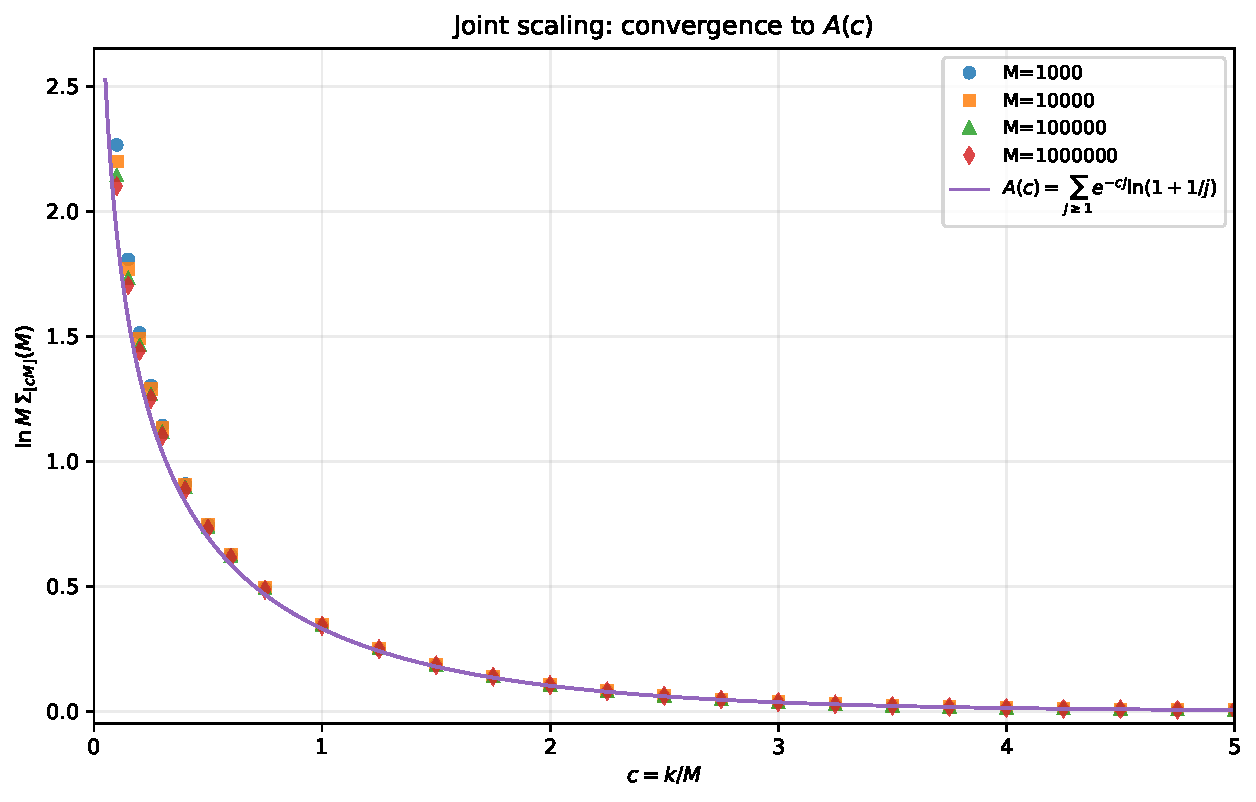
\includegraphics[width=0.85\linewidth]{fig2_joint_scaling.pdf}
\caption{Joint scaling regime $k = \lfloor cM \rfloor$. Points show $\ln M \cdot \Sigma_{\lfloor cM \rfloor}(M)$, evaluated deterministically by direct prime summation in double precision (no Monte Carlo), at $M \in \{10^3, 10^4, 10^5, 10^6\}$. Solid curve: $A(c) = \sum_{j \geq 1} e^{-cj} \ln(1 + 1/j)$, evaluated by adaptive truncation of the positive series when the next term is below $10^{-17}$.}
\label{fig:joint}
\end{figure}

\begin{table}[!htbp]
\centering
\caption{$\ln M \cdot \Sigma_{\lfloor cM \rfloor}(M)$ versus $A(c)$ at $M$ up to $10^7$. Values are evaluated deterministically by direct prime summation and adaptive series truncation in double precision; no Monte Carlo is used. Residuals decay consistently with an $O(1/\ln M)$ next-order strip correction; see text.}
\label{tab:joint}
\small
\begin{tabular}{rrrrrr}
\toprule
$c$ & $A(c)$ & $M = 10^4$ & $M = 10^5$ & $M = 10^6$ & $M = 10^7$ \\
\midrule
0.05 & 2.5267 & 3.0277 & 2.9231 & 2.8498 & 2.7982 \\
0.10 & 1.9095 & 2.1999 & 2.1428 & 2.1009 & 2.0714 \\
0.15 & 1.5688 & 1.7704 & 1.7324 & 1.7033 & 1.6831 \\
0.25 & 1.1687 & 1.2886 & 1.2671 & 1.2498 & 1.2380 \\
0.50 & 0.6954 & 0.7470 & 0.7382 & 0.7307 & 0.7258 \\
0.75 & 0.4665 & 0.4950 & 0.4903 & 0.4861 & 0.4835 \\
1.00 & 0.3301 & 0.3476 & 0.3448 & 0.3422 & 0.3406 \\
1.25 & 0.2406 & 0.2522 & 0.2504 & 0.2486 & 0.2476 \\
1.50 & 0.1787 & 0.1867 & 0.1855 & 0.1843 & 0.1836 \\
2.00 & 0.1020 & 0.1061 & 0.1056 & 0.1049 & 0.1045 \\
3.00 & 0.0356 & 0.0368 & 0.0367 & 0.0365 & 0.0364 \\
5.00 & 0.00469 & 0.00485 & 0.00483 & 0.00480 & 0.00479 \\
7.50 & 0.000384 & 0.000396 & 0.000395 & 0.000393 & 0.000392 \\
10.00 & 0.0000315 & 0.0000325 & 0.0000324 & 0.0000322 & 0.0000321 \\
15.00 & 0.00000021 & 0.00000022 & 0.00000022 & 0.00000021 & 0.00000021 \\
\bottomrule
\end{tabular}
\end{table}

\section{Discussion and Open Problems}\label{sec:discussion}

\emph{Uniform vs.\ non-uniform rates.} Theorem~\ref{thm:sharp-fixed-M} gives an exponential rate at fixed $M$. For $M \geq 11$, the controlling ratio is
\[
\frac{q^{**}(M)}{q^{*}(M)} = \frac{M-3}{M-2} \longrightarrow 1.
\]
Thus the fixed-$M$ bound degenerates as $M \to \infty$ and does not yield the sharp joint-scaling result of Theorem~\ref{thm:joint-sharp}. The joint regime instead requires a uniform argument that combines Lemma~\ref{lem:geom-mean}, decomposition by subset cardinality, and summation over growing $r$.

\emph{Second-order joint asymptotics.} The residuals in Table~\ref{tab:joint} suggest studying an expansion of the form
\[
\ln M\,\frac{\rho_{\lfloor cM\rfloor}(M)-P_M}{P_M}
= A(c)+\frac{B(c)}{\ln M}+o\!\left(\frac{1}{\ln M}\right).
\]
At this scale, both the next-order expansion of the prime-strip sum and the $|T|=2$ component of $R_k(M)$ may contribute. Determining their combined limit and proving that the terms with $|T|\geq 3$ are negligible are left open.

\emph{Second-order fluctuations.} A natural next question is the scale and distributional shape of the fluctuations of $\ln(\varphi(L_k)/L_k)$ about its mean in the same joint regime: the variance asymptotic and an associated central limit theorem. These are developed in separate work in preparation.

\emph{General distributions.} Theorem~\ref{thm:identity} generalises verbatim to any distribution $\mu$ on $\{2, \ldots, M\}$, with $\beta_T(M)$ replaced by $\mu\{n:\gcdop(n,\prod_{p\in T}p)=1\}$. The decomposition and remainder bound in Theorem~\ref{thm:limit-rate} also remain valid after defining $q_p=\mu\{n:p\nmid n\}$. Let $\mathcal{P}_{\mu}:=\{p\leq M:\mu\{n:p\mid n\}>0\}$. Then $\rho_k(M)\to\prod_{p\in\mathcal{P}_{\mu}}(1-1/p)$ as $k\to\infty$. Thus the limit is the full product $P_M$ exactly when $\mathcal{P}_{\mu}=\PM$. A joint scaling limit depends on how the sampling distributions vary with $M$ and is therefore distribution-specific.

\emph{Applications to non-uniform sampling diagnostics.} Departures from uniform sampling change the prime-avoidance probabilities and may deform the joint-scaling function in a distribution-specific way. Quantifying the stability of $A(c)$ under specified perturbation classes could lead to diagnostics for random integer generators over bounded ranges; this requires separate analysis and is left to future work.

\section{Conclusion}\label{sec:conclusion}

We have introduced the expected coprime density $\rho_k(M) = \EE[\varphi(L_k)/L_k]$ of the LCM of random integers in the regime of fixed support and growing sample size, and proved four theorems and one proposition. Theorem~\ref{thm:identity} establishes an exact finite-sum identity over subsets of $\PM$. Theorem~\ref{thm:limit-rate} shows $\rho_k(M) \to P_M$ at fixed $M$ with explicit rate. Theorem~\ref{thm:sharp-fixed-M} sharpens this to a full asymptotic equivalence at fixed $M$, with explicit geometric rate controlled by the ratio $q^{**}(M)/q^*(M)$ of the maximal multi-prime avoidance density to the maximal single-prime avoidance density. Theorem~\ref{thm:joint-sharp} establishes the sharp joint-scaling equivalence $\ln M \cdot (\rho_{\lfloor cM \rfloor}(M) - P_M)/P_M \to A(c) := \sum_{j \geq 1} e^{-cj} \ln(1 + 1/j)$. The uniform control of the multi-prime correction in Theorem~\ref{thm:joint-sharp} comes from combining the elementary bound $\beta_T^k \leq \prod_{p \in T} q_p^{k/|T|}$ with a decomposition by $|T|$ and a summation argument uniform in the subset size. Proposition~\ref{prop:A-asymptotics} gives the $c \to 0^+$ and $c \to \infty$ asymptotics of $A$. Numerical computation up to $M = 10^7$ illustrates Theorem~\ref{thm:joint-sharp}. The regime studied here complements earlier fixed-size tuple, random-subset, and joint-limit models through its i.i.d. sampling-with-replacement formulation and its focus on coprime density; the exact subset identity (Theorem~\ref{thm:identity}) may be of independent use in related problems involving multiplicative functions of random LCMs.

\paragraph{Data and code availability.}
Source code, deterministic seeds, cell-level Monte Carlo errors, and raw numerical output for all figures and tables are available at \url{https://github.com/Wakid90/coprime-density-lcm}. The versioned preprint is archived at \href{https://doi.org/10.5281/zenodo.21325880}{doi:10.5281/zenodo.21325880}.

\begin{thebibliography}{99}

\bibitem{AlsmeyerKabluchkoMarynych2019}
G.~Alsmeyer, Z.~Kabluchko, A.~Marynych, \emph{Limit theorems for the least common multiple of a random set of integers}, Trans.\ Amer.\ Math.\ Soc.\ 372 (2019), 4585--4603.

\bibitem{BostanMarynychRaschel2019}
A.~Bostan, A.~Marynych, K.~Raschel, \emph{On the least common multiple of several random integers}, J.\ Number Theory 204 (2019), 113--133.

\bibitem{BuraczewskiIksanovMarynych2022}
D.~Buraczewski, A.~Iksanov, A.~Marynych, \emph{Central limit theorem for the least common multiple of a uniformly sampled $m$-tuple of integers}, J.\ Number Theory 233 (2022), 301--336.

\bibitem{Cesaro1885}
E.~Ces\`aro, \emph{\'Etude moyenne du plus grand commun diviseur de deux nombres}, Ann.\ Mat.\ Pura Appl.\ 13 (1885), 235--250.

\bibitem{CilleruleoRueSarkaZumalacarregui2014}
J.~Cilleruelo, J.~Ru\'e, P.~\v{S}arka, A.~Zumalac\'arregui, \emph{The least common multiple of random sets of positive integers}, J.\ Number Theory 144 (2014), 92--104.

\bibitem{FernandezFernandez2013}
J.~L.~Fern\'andez, P.~Fern\'andez, \emph{On the probability distribution of the gcd and lcm of $r$-tuples of integers}, arXiv:1305.0536 (2013).

\bibitem{FernandezFernandez2021}
J.~L.~Fern\'andez, P.~Fern\'andez, \emph{Divisibility properties of random samples of integers}, Rev.\ Real Acad.\ Cienc.\ Exactas F\'is.\ Nat., Ser.\ A Mat.\ 115 (2021), article 26.

\bibitem{HilberdinkToth2016}
T.~Hilberdink, L.~T\'oth, \emph{On the average value of the least common multiple of $k$ positive integers}, J.\ Number Theory 169 (2016), 327--341.

\bibitem{IksanovMarynychRaschel2022}
A.~Iksanov, A.~Marynych, K.~Raschel, \emph{Asymptotics of arithmetic functions of GCD and LCM of random integers in hyperbolic regions}, Results Math.\ 77 (2022), article 165.

\bibitem{KabluchkoMarynychRaschel2023}
Z.~Kabluchko, A.~Marynych, K.~Raschel, \emph{Multivariate multiplicative functions of uniform random vectors in large integer domains}, Results Math.\ 78 (2023), article 201.

\bibitem{Lichtman2021}
J.~D.~Lichtman, \emph{Mertens' prime product formula, dissected}, Integers 21A (2021), article A17.

\bibitem{Ramanujan1919}
S.~Ramanujan, \emph{A proof of Bertrand's postulate}, J.\ Indian Math.\ Soc.\ 11 (1919), 181--182.

\bibitem{RosserSchoenfeld1962}
J.~B.~Rosser, L.~Schoenfeld, \emph{Approximate formulas for some functions of prime numbers}, Illinois J.\ Math.\ 6 (1962), 64--94.

\bibitem{Sanna2021}
C.~Sanna, \emph{On the least common multiple of random $q$-integers}, Res.\ Number Theory 7 (2021), article 16.

\bibitem{Tenenbaum2015}
G.~Tenenbaum, \emph{Introduction to Analytic and Probabilistic Number Theory}, 3rd ed., Graduate Studies in Mathematics 163, Amer.\ Math.\ Soc., 2015.

\end{thebibliography}

\end{document}
